\documentclass[a4paper,12pt]{article}

\usepackage{geometry}
\usepackage{cmap}
\usepackage{enumerate}
\usepackage[russian]{babel}
\usepackage{listings}
\usepackage{verbatim}
\usepackage{pdfpages}
\usepackage[font=small,labelfont=bf]{caption}

\geometry{a4paper, left=20mm, right=10mm, top=20mm, bottom=20mm}

\lstdefinestyle{cppcode}{
	basicstyle=\ttfamily
}

\lstset{language=C++,style=cppcode}

\begin{document}
		
\begin{titlepage}		

\begin{center}
	\textsc{\textbf{Правительство Российской Федерации}}\\
	\vspace{0.5cm}
	\hrule
	\vspace{0.5cm}
	\textsc{Федеральное государственное автономное образовательное учреждение высшего образования <<Национальный исследовательский университет <<Высшая школа экономики>>}\\
	\vspace{1cm}
	Кафедра <<Компьютерная безопасность>>
\end{center}	

\vspace{\fill}

\begin{center}
	\Large{\textbf{ОТЧЕТ \\ К ЛАБОРАТОРНОЙ РАБОТЕ №1}} \\
	\vspace{1em}
	\textbf{по дисциплине} \\
	\vspace{1em}
	\large{\textbf{<<Языки программирования>>}}
\end{center}

\vspace{\fill}

\begin{flushright}
	\begin{minipage}[center]{15cm}
		\begin{minipage}[left]{5cm}
			{Работу выполнил\\студент группы СКБ-203}
		\end{minipage}
		\begin{minipage}[center]{5cm}
			\vspace{1.25cm}
			\hrulefill\\[-1cm]
			\begin{center}{подпись, дата}\end{center}
		\end{minipage}
		\begin{minipage}[right]{4cm}
			\vspace{0.4cm}
			\begin{flushright}{К.А. Павкин}\end{flushright}
		\end{minipage}
		\\
		\\
		\\
		\begin{minipage}[left]{5cm}
			{Работу проверил}
		\end{minipage}
		\begin{minipage}[center]{5cm}
			\vspace{1.25cm}
			\hrulefill\\[-1cm]
			\begin{center}{подпись, дата}\end{center}
		\end{minipage}
		\begin{minipage}[right]{4cm}
			\begin{flushright}{С.А. Булгаков}\end{flushright}
		\end{minipage}
	\end{minipage}
\end{flushright}

\vspace{\fill}

\begin{center}
	Москва~2021
\end{center}

\end{titlepage}

\tableofcontents
\cleardoublepage

\section*{<<Пользовательский тип>>}\addcontentsline{toc}{section}{Постановка задачи}

Разработать программу на языке Си++ (ISO/IEC 14882:2014), демонстрирующую решение поставленной задачи.

\subsection*{Постановка задачи}

Разработать набор классов, объекты которых реализуют типы данных, указанные ниже.
Для классов разработать необходимые конструкторы, деструктор, конструктор копирования, а также методы, обеспечивающие изменение отдельных составных частей объекта.
Используя перегрузку операторов (operator) разработать стандартную арифметику объектов, включающую арифметические действия над объектами и стандартными типами (целыми, вещественными, строками – в зависимости от вида объектов), присваивание, ввод и вывод в стандартные потоки (используя операторы <<\verb!<<!>> и <<\verb!>>!>>), приведение к/от базового типа данных.
Организовать операции в виде конвейера значений, с результатом (новым объектом) и сохранением значений входных операндов.

\subsubsection*{Задачи}

\begin{enumerate}
	
\item
Дата и время, представленные целочисленными переменными: год, месяц, день, час, минута, секунда.
Базовый тип: \verb!uint64_t! формат представления unix time.
Реализовать возможность преобразования в/из формата представления filetime.

\item
Целое произвольной длины (во внешней форме представления в виде строки символов-цифр).
Базовый тип: \verb!std::string!.

\item
Год <<от Адама>>, имеющий внутреннее представление в виде целочисленных переменных: индикт, круг солнцу, круг луне.
Диапазоны значений (циклические): индикт 1—15, круг солнцу 1—28, круг луне 1—19.
Ежегодно каждая переменная увеличивается на 1.
Итоговое значение вычисляется как произведение переменных.
Необходима возможность отображения/задания как в виде одного числа, так и виде трех.
Реализовать возможность преобразования в/из формата представления <<от рождества Христова>> используя соответствие 1652 = 7160 <<от Адама>>.

\item Разреженная матрица, представленная динамическим массивом структур, содержащих описания ненулевых коэффициентов: индексы местоположения коэффициента в матрице (целые) и значение коэффициента (вещественное).
	
\end{enumerate}

\cleardoublepage

\section{Алгоритм решения задачи}

В процессе анализа предметной области были выявлены основные алгоритмы, необходимые для реализации всеобъемлющей, асимптотически эффективной и отлаженной программы для решения поставленной задачи.

\subsection{Дата и время}

Учитывая формат представления даты в времени, становится заметен ньанс при написании валидации аргументов сеттера для дня.
Дело в том, что максимальное значение месяца в февраля не является константным.
Появляется необходимость понять, является ли год високосным.
Более того, как будет известно далее, полезно также знать, сколько лет в некотором диапазоне были високосными.
Для этого были написаны функции из листинга \ref{lst1}.

\begin{lstlisting}[caption={Функции для работы с високосными годами},captionpos=b,label=lst1]

int date::leap_years_until(int year)
{
	return year / 4 - year / 100 + year / 400;
}

int date::leap_years_between(int start, int end)
{
	return leap_years_until(end) - leap_years_until(start - 1);
}

bool date::is_leap_year(int year)
{
	return leap_years_between(year, year) == 1;
}

\end{lstlisting}

Перевод из/в формат представления unix time было решено вычислять без использования каких-либо библиотек.
Посчитав количество лет с начала 1970 года, становится возможным рассчитать количество дней, прошедших с начала текущего года.
По аналогии рассчитывается количество секунд, прошедших с начала дня.\\


Перевод из/в формат представления file time имеет несущественные различия по отношению к уже написаннымм преобразованями.

\subsection{Целое произвольной длины}

Целое число произвольной длины, позволяющее работать с числами без ограничений, было решено хранить в виде динамического массива битов (булевых переменных), где крайний правый бит отвечает за знак.
Такое решение позволяет свести к минимуму простои памяти, а также даёт возможность поддерживать побитовые операции с привычной для них логикой.
В процессе разработки библиотеки был реализован широкий спектр побитовых, арифметических и логических операторов, а также полная, бесшовная совместимость со встроенным типом \verb!int!.\\

Если побитовые операции были реализованы практически нативно, с поэлементным применением логических операторов к двум соседним битам двух чисел, то арифметические операции, основываясь на побитовых, уже требовали базовых знаний математики для сложения, умножения и деления <<в столбик>>.\\

При примении бинарного оператора к числам, имеющим различную вместительность, вызывется функция \verb!resize! в отношении числа с меньшей вместительностью, которая его увеличивает.
Данная функция представлена в листинге \ref{lst2}.

\begin{lstlisting}[caption={Функция, меняющая вместительность числового типа},captionpos=b,label=lst2]
	
void number::resize(size_t capacity)
{
	bool* new_binary = new bool[capacity];
	
	size_t min = std::min(this->capacity, capacity);
	
	for (size_t i = 0; i < min - 1; i++) {
		new_binary[i] = binary[i];
	}
	
	for (size_t i = min - 1; i < capacity; i++) {
		new_binary[i] = binary[this->capacity - 1];
	}
	
	this->capacity = capacity;
	
	binary = new_binary;

	delete[] new_binary;
}
	
\end{lstlisting}

Код выше создаёт число с новой вместительностью, копирует в него все элементы из старого, а оставшееся место заполняет значением знака.
Последнее действие необходимо для поддержания знака числа при изменении его вместительности.
Минимальное значение вместительности ограничено 32 битами.\\

Отдельного внимания требует логика вычислений: вместительность числа \textbf{не пересчитывается} в процессе выполнения какого-либо оператора.
Таким образом, класс не нивелирует опасность переполнения типа в случае, например, перемножения слишком больших чисел.
Для контроля переполнения в классе предусмотрена функция \verb!get_capacity!, возвращающая текущую вместительность числа.\\

Вдумчивый читатель уже заметил ощутимый недостаток от подобного решения, заключающийся в том, что двоичное число нельзя побитово перевести в строку и вывести в поток вывода.
Пользователям просто непривычен двоичный формат представления чисел.
Для перевода в десятичную систему счисления предусмотрены закрытые функции сложения двух строк и деления строки на два, пользующиеся спросом у операторов чтения и записи.

\subsection{Год <<от Адама>>}

Год <<от Адама>> — система летоисчисления <<от сотворения мира>> (начинается с 5508 года до н. э.).
В качестве представления было предложено использовать независимые переменные: индикт (1—15), круг солнцу (1—28) и круг луне (1—19).
Ежегодно каждая переменная увеличивается на единицу, и, превышая заданный диапазон, сбрасывается до первоначального состояния.\\

Таким образом, год <<от Адама>> вычисляется как решение системы линейных алгебраических уравнений по трём переменным, в частности, с использованием китайской теоремы об остатках (см. листинг \ref{lst3}).

\begin{lstlisting}[caption={Алгоритм нахождения года <<от Адама>>},captionpos=b,label=lst3]
	
int adam::to_adam_year() const
{
	int m1 = MAX_ADAM_YEAR / 15, y1;
	int m2 = MAX_ADAM_YEAR / 28, y2;
	int m3 = MAX_ADAM_YEAR / 19, y3;
	
	for (int y = 0, m = m1 % 15; y < 15; y++)
		if ((m * y) % 15 == indict)
			y1 = y;
	for (int y = 0, m = m2 % 28; y < 28; y++)
		if ((m * y) % 28 == sun)
			y2 = y;
	for (int y = 0, m = m3 % 19; y < 19; y++)
		if ((m * y) % 19 == moon)
			y3 = y;
	
	return (m1 * y1 + m2 * y2 + m3 * y3) % MAX_ADAM_YEAR;
}

\end{lstlisting}

Сами же переменные вычисляются как остаток от деления года <<от Адама>> на 15, 28 и 19 соответственно.

\subsection{Разреженная матрица}

Разреженной матрицей называют такую матрицу, которая наполнена преимущественно нулевыми элементами.
Для такой матрицы наиболее оптимальным способом хранения является так называемый список смежности, где для каждой строки существуют только заполненные значения в соответствующих колонках — \verb!map<size_t, double>[]!.
В процессе вычислений итерация происходит не по всем элементам матрицы, а лишь по заполненным, что является асимтотически эффективным решением поставленной задачи.\\

Помимо базовых операций с матрицами были реализованы операторы сложения и умножения матриц, оператор умножения матрицы на число, функции для получения определителя, обратной и транспонированной матрицы.
В логических операторах учтены ньансы при работе с типом double — для равенства двух переменных модуль их разницы должен быть меньше 1e-6.

\cleardoublepage

\section{Выполнение задания}

На рисунке \ref{pic1} представлена диаграмма классов, демонстрирующая формат хранения данных, а также критически важные методы.
В целях сужения диаграммы, операторы и некоторые функции были опущены.
Зависимостей между классами нет.

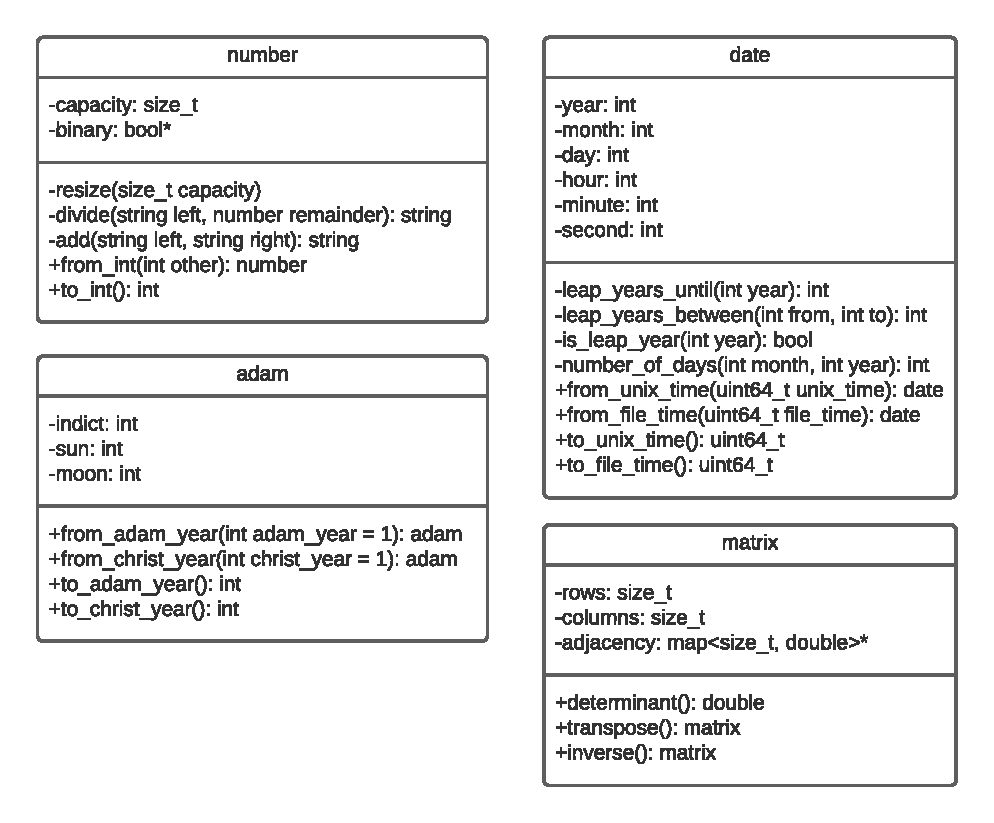
\includegraphics{UML Class.pdf}

\captionof{figure}{Диаграмма классов}\label{pic1}

~\\

Заголовочные файлы созданных библиотек приведены в приложении А.

\begin{enumerate}

\item Дата и время — \verb!date.h!\ref{att1}

\item Целое произвольной длины — \verb!number.h!\ref{att2}

\item Год <<от Адама>> — \verb!adam.h!\ref{att3}

\item Разреженная матрица — \verb!matrix.h!\ref{att4}
	
\end{enumerate}

\cleardoublepage

\section{Получение исполняемых модулей}

Заголовочные файлы и их реализации были размещены в различных директориях. Для сборки проекта в каждую директорию были помещены файлы CMakeLists.txt, и, таким образом, каждая директория представляет из себя отдельную библиотеку, которая в последствии собирается в корневом каталоге. Файл сборки CMakeLists.txt из корневого каталога показан в приложении А.\ref{att5}

\cleardoublepage

\section{Тестирование}

Файл \verb!main.cpp! содержит юнит-тесты, целью которых является сравнение ожидаемых от функций значений с фактическими, и выдача оповещений при их несовпадении.

\subsection{Прецеденты для класса date}

\begin{enumerate}

\item unix\_time\_conversion — проверяет коррентность преобразований из/в формат представления unix time (количество секунд, прошедших с начала 1970 года)

\item file\_time\_conversion — проверяет коррентность преобразований из/в формат представления file time (количество интервалов по 100 наносекунд, прошедших с начала 1601 года)
	
\item addition — проверяет коррентность сложения даты с числом или другой даты

\item subtraction — проверяет коррентность вычитания из даты числа или другой даты

\item increment — проверяет коррентность инкрементов

\item decrement — проверяет коррентность декрементов

\end{enumerate}

\subsection{Прецеденты для класса number}

\begin{enumerate}

\item string\_conversion — проверяет коррентность преобразования из/в строковый (десятичный) формат представления \verb!std::string!

\item int\_conversion — проверяет коррентность преобразования из/во встроенный числовой тип \verb!int!

\item bitwise\_not — проверяет корректность унарного оператора побитового НЕ

\item bitwise\_and — проверяет корректность оператора побитового И в отношении другого числа (number) или встроенного типа \verb!int!

\item bitwise\_or — проверяет корректность оператора побитового ИЛИ в отношении другого числа (number) или встроенного типа \verb!int!

\item bitwise\_xor — проверяет корректность оператора побитового исключающего ИЛИ в отношении другого числа (number) или встроенного типа \verb!int!

\item bitwise\_left\_shift — проверяет корректность оператора побитового сдвига влево в отношении другого числа (number) или встроенного типа \verb!int!

\item bitwise\_right\_shift — проверяет корректность оператора побитового сдвига вправо в отношении другого числа (number) или встроенного типа \verb!int!

\item unary\_minus — проверяет корректность унарного оператора минус

\item addition — проверяет корректность оператора сложения в отношении другого числа (number) или встроенного типа \verb!int!

\item subtraction — проверяет корректность оператора вычитания в отношении другого числа (number) или встроенного типа \verb!int!

\item multiplication — проверяет корректность оператора умножения в отношении другого числа (number) или встроенного типа \verb!int!

\item division — проверяет корректность оператора деления в отношении другого числа (number) или встроенного типа \verb!int!

\item modulo — проверяет корректность оператора взятия остатка от деления в отношении другого числа (number) или встроенного типа \verb!int!

\item increment — проверяет коррентность инкрементов

\item decrement — проверяет коррентность декрементов

\end{enumerate}

\subsection{Прецеденты для класса adam}

\begin{enumerate}
	
\item adam\_year\_conversion — проверяет коррентность преобразований из/в формат представления <<год от Адама>>

\item christ\_year\_conversion — проверяет коррентность преобразований из/в формат представления <<год от рождества Христова>>

\item addition — проверяет коррентность сложения года с числом или другим годом

\item subtraction — проверяет коррентность вычитания из года числа или другого года

\item increment — проверяет коррентность инкрементов

\item decrement — проверяет коррентность декрементов
	
\end{enumerate}

\subsection{Прецеденты для класса matrix}

\begin{enumerate}
	
\item string\_conversion — проверяет коррентность преобразования из/в строковый (десятичный) формат представления \verb!std::string!
	
\item identity — проверяет корректность получения единичной матрицы

\item determinant — проверяет корректность вычисления определителя матрицы

\item transpose — проверяет корректность получения транспонированной матрицы

\item inverse — проверяет корректность получения обратной матрицы

\item unary\_minus — проверяет корректность унарного оператора минус

\item addition — проверяет коррентность сложения матриц

\item subtraction — проверяет коррентность вычитания матриц

\item matrix\_multiplication — проверяет коррентность умножения матриц

\item number\_multiplication — проверяет коррентность умножения матрицы на число
	
\end{enumerate}

\cleardoublepage

\section*{Приложение А}\addcontentsline{toc}{section}{Приложение А}

\subsection*{Файл {\tt date.h}}\label{att1}

\verbatiminput{../date/date.h}
\cleardoublepage

\subsection*{Файл {\tt date.cpp}}\label{att6}

\verbatiminput{../date/date.cpp}
\cleardoublepage

\subsection*{Файл {\tt  number.h}}\addcontentsline{toc}{subsection}{Файл number.h}\label{att2}

\verbatiminput{../number/number.h}
\cleardoublepage

\subsection*{Файл {\tt  number.cpp}}\label{att7}

\verbatiminput{../number/number.cpp}
\cleardoublepage

\subsection*{Файл {\tt adam.h}}\addcontentsline{toc}{subsection}{Файл adam.h}\label{att3}

\verbatiminput{../adam/adam.h}
\cleardoublepage

\subsection*{Файл {\tt adam.cpp}}\label{att8}

\verbatiminput{../adam/adam.cpp}
\cleardoublepage

\subsection*{Файл {\tt matrix.h}}\addcontentsline{toc}{subsection}{Файл matrix.h}\label{att4}

\verbatiminput{../matrix/matrix.h}
\cleardoublepage

\subsection*{Файл {\tt matrix.cpp}}\label{att9}

\verbatiminput{../matrix/matrix.cpp}
\cleardoublepage

\subsection*{Файл {\tt CMakeLists.txt}}\addcontentsline{toc}{subsection}{Файл CMakeLists.txt}\label{att5}

\verbatiminput{../CMakeLists.txt}
\cleardoublepage

\end{document}